\chapter{Maintaining Room State \\
  \small{\textit{-- Evan Ciok, Sophia DiCuffa, Carson McManus}}
  \index{Chapter!room-state}
  \label{Chapter::RoomState}}

\section{Lost Balancer-Monolith Connections}

When a Balancer-Monolith connection is lost, clients connected to that monolith need to be handled appropriately. Otherwise, the accuracy of room state is compromised. 
All client connections that are in rooms on the lost monolith are no longer valid, so they need to be disconnected and removed 
from their rooms. From there, they can reconnect to a monolith with a new websocket connection to the balancer. 

\section{Duplicate Rooms Across Monoliths}

Two monolith nodes should never have the same room loaded, as the load balancer should be directing all connections for a given room to the designated monolith using its preserved states. 
In the case that this does happen, the system is then in a bad state and it must be resolved. The planned solution to this issue is to have the load balancer unload rooms that were not the 
first instance of that particular room. This means that the duplicate instances would be unloaded and the clients could then rejoin the room in a healthy state. In order to accomplish this, 
every room must have a timestamp associated with it, designating the time it was loaded. Then, in the case of duplication, the timestamps can be compared and the more recently loaded 
instances can be handled appropriately. Following this, clients who were connected to a bad load of a room should be redirected to the home page where they can enter a new flow of room 
creation or room joining. 

\begin{figure}[!htb]
  \centering
  \scalebox{0.57}{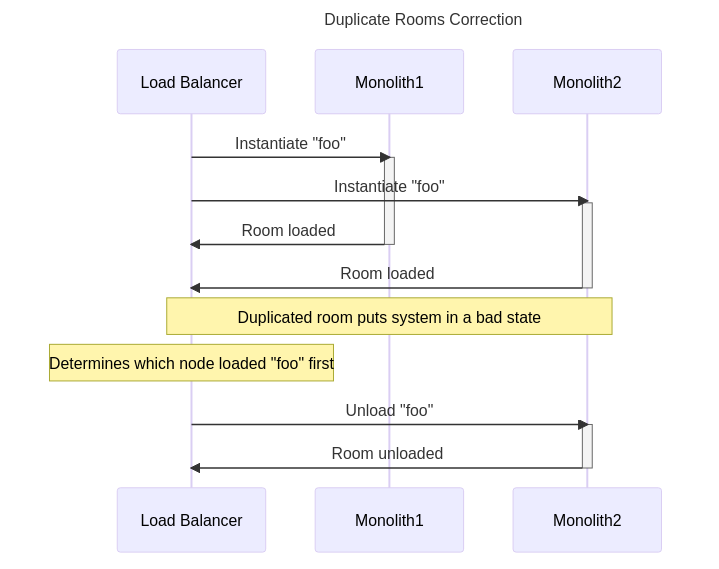
\includegraphics{Figures/duplicate-rooms.png}}
  \caption{\label{Figure::duplicate-rooms} Correcting system state following duplicate room instances.}
\end{figure}